\chapter{Real dataset}
\label{sec:aviloo_ds}

\section{Data acquisition}
\label{sec:aviloo_ds_intro}
To further expand our collection of EV monitoring data and in order to parametrize our Simulink EV model correctly (sec. \ref{sec:parameter_estimation}), two datasets of real EV field measurements were acquired from a private EV fleet management company (sec. \ref{sec:aviloo}). The datasets span several months of data acquisition from a VW e-up! and a VW e-Golf. Many battery SOH tests were performed throughout the monitored time periods, as reported in the next section.

\begin{figure}[htb!]
\centering
\begin{subfigure}[t]{0.475\textwidth}
    \centering
    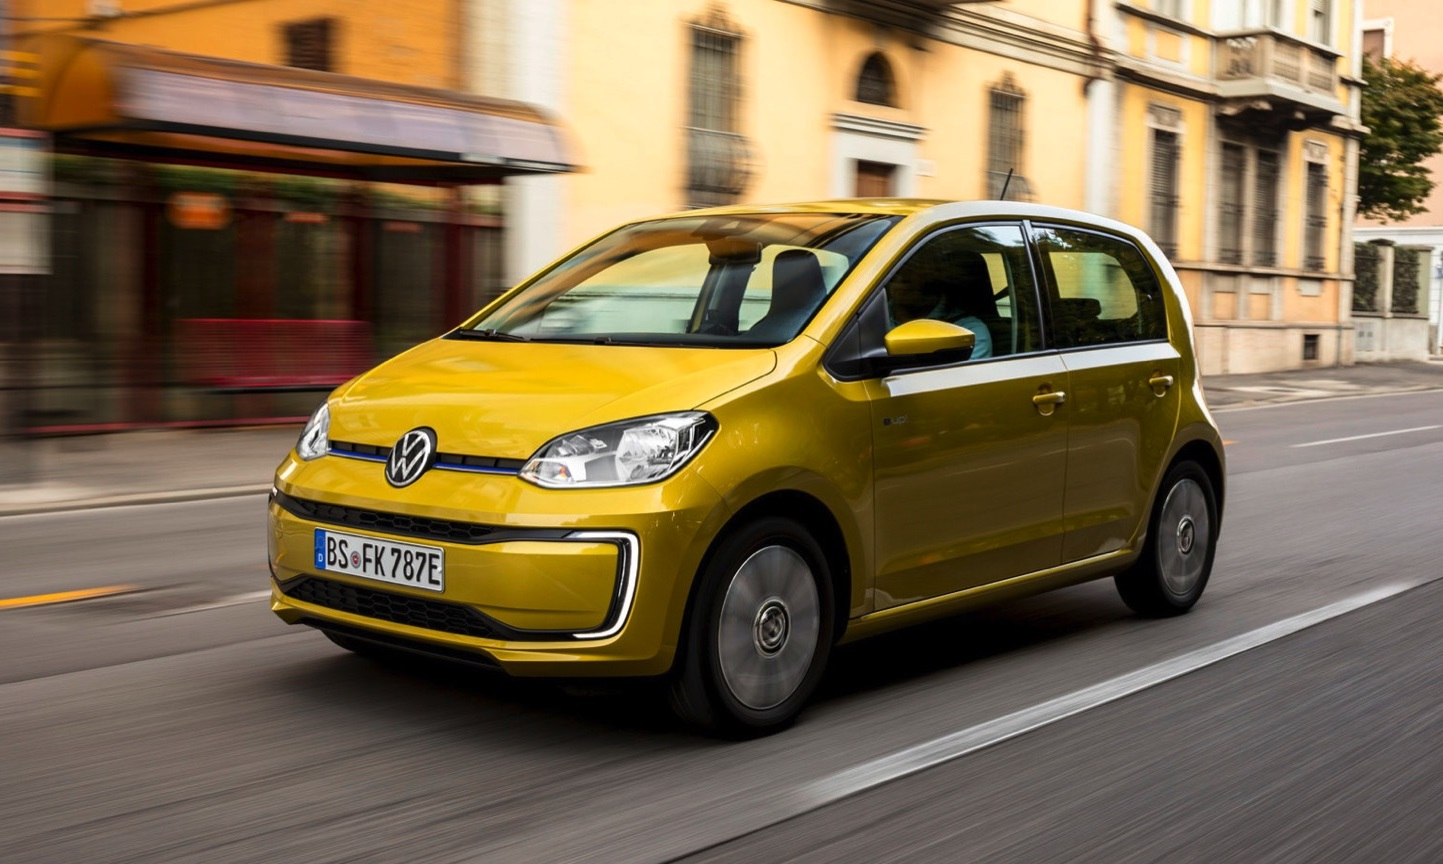
\includegraphics[width=\textwidth]{images/eup}
    \caption{VW e-up!}
\end{subfigure}
\hfill
\begin{subfigure}[t]{0.475\textwidth}
    \centering
    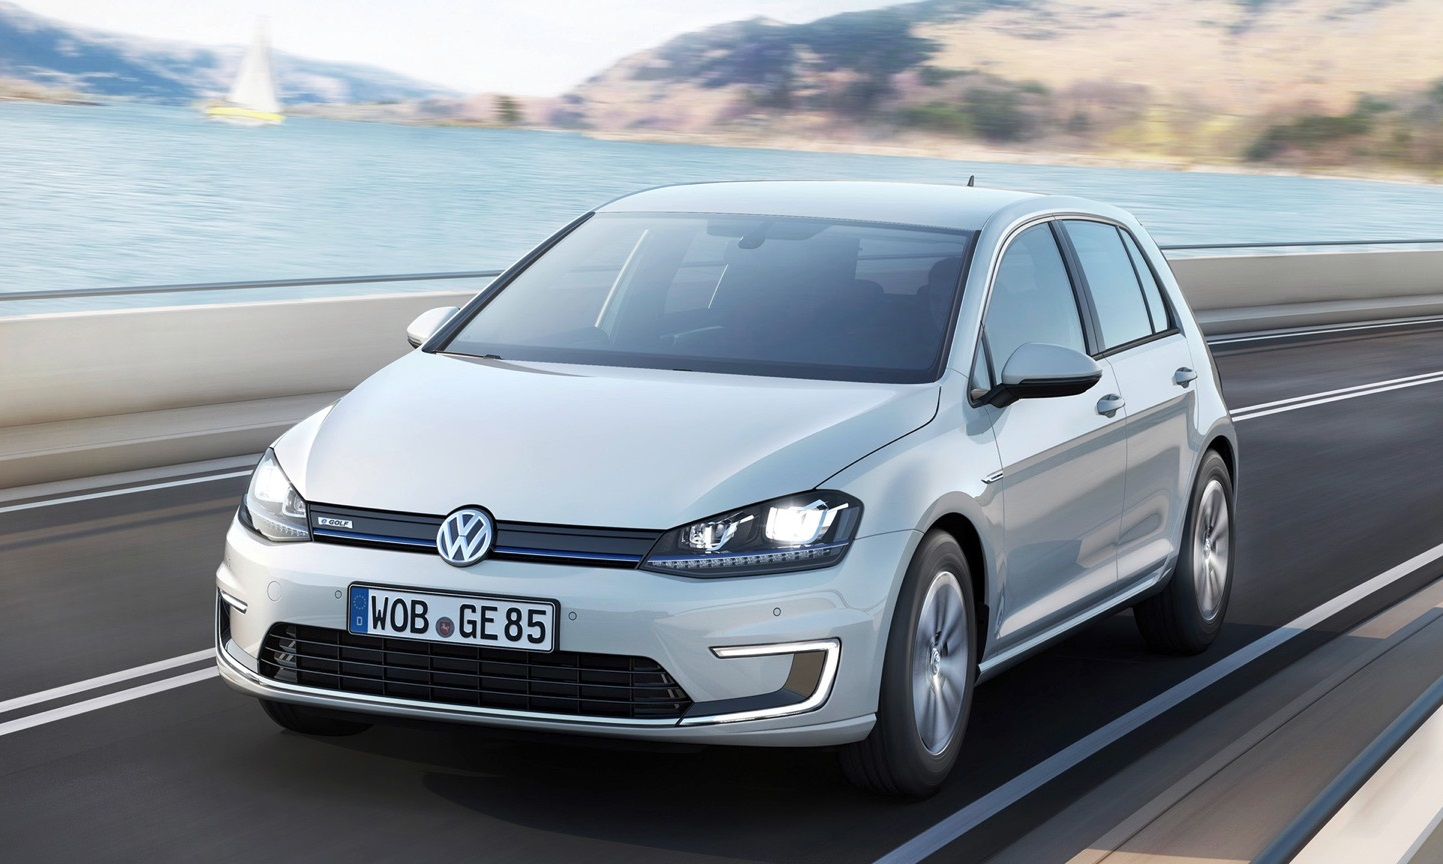
\includegraphics[width=\textwidth]{images/egolf}
    \caption{VW e-Golf}
\end{subfigure}
\caption[VW e-up! and VW e-Golf]{The two Volkswagen EV models monitored by the private EV fleet management company.}
\label{fig:eup_egolf}
\end{figure}



\section{Data exploration}
\label{sec:aviloo_ds_exploration}
The two vehicles were monitored over different time periods\footnote{dates are in dd/mm/yyyy format}:
\begin{itemize}
    \item e-up!: 20/10/2021 - 18/12/2021
    \item e-Golf: 04/06/2019 - 12/06/2019, 27/06/2019 - 22/10/2020, 16/11/2020 - 07/12/2020, 15/02/2021 - 10/03/2021, 06/04/2021 - 10/05/2021, 12/07/2021 - 07/09/2021
\end{itemize}

Battery tests were performed over the monitored time periods for both models. The e-up! underwent a single battery test on 06/12/2021, which returned an SOH of 88\%. The e-Golf underwent 16 battery tests, whose dates and returned SOH values are reported in tab. \ref{tab:egolf_bchecks} for convenience.

\begin{table}[htb!]
\centering
\begin{tabular}[t]{cc}
\toprule
Test date & SOH(\%)\\
\midrule
22/07/2020 & 95\\
10/09/2020 & 95\\
23/11/2020 & 95\\
29/11/2020 & 93\\
17/02/2021 & 94*\\
08/03/2021 & 95\\
26/04/2021 & 95\\
03/05/2021 & 95\\
\bottomrule
\end{tabular}
\hspace{1cm}
\begin{tabular}[t]{cc}
\toprule
Test date & SOH(\%)\\
\midrule
08/07/2021 & 93\\
12/07/2021 & 95\\
16/08/2021 & 93\\
23/08/2021 & 95\\
15/09/2021 & $>100$*\\
02/11/2021 & 89*\\
05/11/2021 & 93*\\
22/11/2021 & 91*\\
\bottomrule
\end{tabular}
\caption[Battery tests performed on the monitored VW e-Golf]{Battery tests performed on the monitored VW e-Golf. Asterisk marks (*) indicate that the battery test doesn't fulfill the standard conditions for a reliable SOH estimation (i.e. driving the car from $100\%$ SOC to $<10\%$ SOC, as discussed in sec. \ref{sec:aviloo}), thus the estimated SOH value might not reflect the actual one precisely. The estimated SOH values have a maximum error of $\pm 1.5$, as claimed by the private EV fleet management company from whom the data was acquired.}
\label{tab:egolf_bchecks}
\end{table}

Training a machine learning algorithm for the real-time on-board SOH estimation requires having extensive monitoring data collected at different SOH levels. Unfortunately, the estimated SOH values during the monitored time periods exhibit very little variability. Therefore, e-up! and e-Golf real datasets will be used only for evaluating the performances of the proposed SOH estimation procedure (sec. \ref{sec:results}). To make the two datasets suitable for testing, only data of driving sessions associated to known battery test SOH values may be selected. We will make the assumption that data spanning from one week before and one week after a battery test (where available\footnote{As evident from tab. \ref{tab:egolf_bchecks}, there are some battery tests which were performed outside of the monitored time periods, therefore no monitoring data is available close in time to them}) is associated with the SOH value returned by that battery test. Whenever two contiguous battery tests were performed less than two weeks away from each other, less than a week of monitoring data is selected after or before those battery tests, in order to avoid any overlapping.

The provided monitoring data is characterized by many signals, whose measurements were collected by the BMS of the EV at different sampling rates and read by a monitoring device through the OBD port. The signals monitored by the BMS vary among different EV models; however, being designed from the same manufacturer, the VW e-up! and VW e-Golf have almost the same set of monitored signals. A complete list of all the common signals between the e-up! and the e-Golf is reported in tab. \ref{tab:aviloo_signals}.

\begin{table}[htb!]
\scriptsize
\centering
\begin{tabular}[t]{lll}
\toprule
Signal name & Description & \breakcellleft{Avg. sampling\\rate (s)}\\
\midrule
CUMULATIVE\_CC & Cumulative charged charge [C] & 33\\
CUMULATIVE\_CE & Cumulative charged energy [J] & 33\\
CUMULATIVE\_DC & Cumulative discharged charge [C] & 33\\
CUMULATIVE\_DE & Cumulative discharged energy [J] & 33\\
CURRENT & Current flowing through the pack [A] & 0.15, 0.1\\
ENERGY\_REMAINING\_EXPECTED & Remaining energy (expected) [J] & 23\\
IGNITION & Whether the vehicle is on (1) or off (0) & 7\\
MILEAGE & Mileage [km] & 17\\
SERIAL\_BATTERY & Serial number of the pack (string) & 100\\
SOC\_DISPLAY & Displayed SOC(\%) & 7\\
SOC\_REAL & Actual SOC(\%) & 7\\
SPEED & Speed [km/h] & 13, 19\\
T\_CELL\_AVG & Average cell temperature [°C] & 12\\
T\_CELL\_MAX & Maximum cell temperature [°C] & 12\\
T\_CELL\_MIN & Minimum cell temperature [°C] & 12\\
T\_MODULE\_$n$ & Temperature of the $n$-th module [°C] & 13, 4\\
T\_OUTSIDE & External temperature [°C] & 100, 14\\
VOLTAGE & Terminal voltage of the pack [V] & 0.15, 0.1\\
VOLTAGE\_12V & Terminal voltage of the ignition battery [V] & 21\\
VOLTAGE\_CELL\_$n$ & Terminal voltage of the $n$-th cell [V] & 1\\
VOLTAGE\_CELL\_MAX & Maximum cell terminal voltage [V] & 1\\
VOLTAGE\_CELL\_MAX\_NUMBER & Cell with the highest terminal voltage & 1\\
VOLTAGE\_CELL\_MIN & Minimum cell terminal voltage [V] & 1\\
VOLTAGE\_CELL\_MIN\_MUMBER & Cell with the lowest terminal voltage & 1\\
VOLTAGE\_CONN & Voltage at the connector [V] & 0.15, 0.1\\
\bottomrule
\end{tabular}
\caption[Signals monitored by the BMS]{Signals monitored by the BMS and read by a monitoring device through the OBD port. When sampling rates are different between the two models, the e-up! sampling time is reported first. In both datasets there is no invalid data; however "SPEED" measurements are missing in some e-Golf driving sessions.}
\label{tab:aviloo_signals}
\end{table}

The e-up! data was provided directly on a proprietary online platform, in a format which makes it easy to explore and manage the data. Data associated with each driving session can be selected and downloaded in csv format directly from the platform. On the other hand, the e-Golf data was provided in raw csv files, from which it was difficult to tell different driving sessions apart. Moreover, "SPEED" measurements are missing in some of these files. Therefore, in this case, driving sessions have been manually identified and extracted with the following procedure:
\begin{itemize}
    \item where the "SPEED" measurements are available, a driving session corresponds to the time interval from the first sampled non-zero speed value to the last one, with sub-intervals of at most five minutes in which speed may be zero.
    \item where the "SPEED" measurements are not available, a driving session corresponds to the time interval from the first increase in "MILEAGE" value to the last one, with sub-intervals of at most five minutes in which mileage may not increase.
\end{itemize}

\noindent The csv files containing driving session data have rows formatted as
\[
\text{\texttt{Timestamp, Timestamp (Unix Microseconds), Signal Type, Value}}
\]
For our aims, only "SPEED", "VOLTAGE", "CURRENT", "SOC\_REAL" and "TEMPERATURE" signals are selected. Specifically: "SPEED" is needed to add real drive cycles to \texttt{DC\_LIST} for the synthetic dataset generation (sec. \ref{sec:ds_gen}); "VOLTAGE", "CURRENT", "SOC\_REAL" and "TEMPERATURE" are needed to parametrize Simulink's GBM block (sec. \ref{sec:parameter_estimation}) and -- with the exception of "TEMPERATURE" -- to test the performances of the proposed SOH estimation procedure (chap. \ref{sec:experiments}). The resulting dataset of extracted driving sessions, each associated to a known SOH level, will undergo further cleaning and preprocessing steps in sec. \ref{sec:ds_preprocessing}.

At a later time, a further set of battery test field data for six different e-Golf vehicles became available, with associated SOH values: 93\%, 94\%, 99\%, 94\%, 96\%, 98\%. They were acquired as raw csv files and processed as already explained. Finally, they were concatenated to the existing e-Golf driving sessions dataset.